\chapter{Metoder}
Afsnittet indeholder en beskrivelse af hvilke metoder, der er blevet anvendt til udarbejdelse af denne mini-MTV i forhold til de fire MTV aspekter: Teknologi, Organisation, Patient og Økonomi.

Overordnet set er der blevet gennemført en litteratursøgning og -vurdering på baggrund af en i forvejen opstillet protokol, se Bilag 11. Protokollen er udarbejdet ud fra specifikke søgestrategier, hvor der er søgt på både engelsk og dansk. De specifikke søgeord er medtaget som dokumentation. Der er søgt i følgende databaser: Embase, PubMed, Google Scholar, Cochrane og Engineering Village. 

Generelt har det været et problem at finde videnskabelige artikler til alle afsnit i rapporten undtagen til Organisation. Videnskabelige artikler omhandlende arbejdsskader har været relativt nemme at fremsøge, dog har det ikke været muligt at finde relevant litteratur til Økonomiafsnittet. Endvidere har det været nødvendigt at gøre egne erfaringer for at få et indblik i organisationen og patientoplevelsen på HEH og RMV, samt teknologien bag Ultralyds Robotarmen. Metoden semi-struktureret interview blev benyttet til at indhente oplysninger fra HEH og RMV. \\ 
De fremsøgte artikler er blevet sorteret ud fra inklusions- og eksklusionskriterier, se figur \ref{InklusionEksklusion}. 

\begin{figure}[H]\centering
	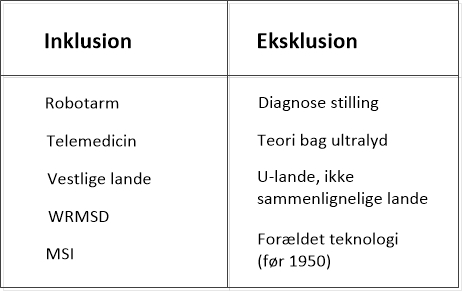
\includegraphics[width = 0.6\textwidth]{Figurer/InklusionEksklusion}
	\caption{Inklusion- og eksklusionkriterier ved litteratursøgning}
	\label{InklusionEksklusion}
\end{figure}

Dermed er artikler omhandlende scanning af gravide, scanning af hjertet, robotarm og arbejdsskader hos sonografer er inkluderet i mini-MTV'en.\\
Udover ovenstående litteratur er der, efter behov søgt efter ikke videnskabelig litteratur for at opnå en forståelse for opbygningen af sonograf uddannelse, ultralydsscanning og andre løse emner for at komme ind i problemstillingen. 

\section{Teknologi}
Dataindsamling til Teknologiafsnittet er sket via antagelser fra CEO Søren Pallesen, Robotic Ultrasound ApS, produktspecifikationer fra Universal Robots, samt information fra interview og samtale med sonografer på HEH og RVM. Det var ønsket at data indsamlingen til Teknologiafsnittet var via videnskabelige artikler der underbyggede brugen af ultralyds Robotarmen til kompliceret scanninger og scanninger af gravide med højt BMI. \\ 
Endvidere skulle videnskabelige artikler skabe evidens for sikkerhedsindstillingen på 5 kg og tekniske specifikationer for trykfeedback i dummy-proben. Data indsamlet fra interview belyser det nuværende udstyr på afdelingerne, da ultralyds Robotarmen er en add-on løsning til det eksisterende. Afsnittet belyser Ultralyds Robotarmens anvendelsesområder, specifikationer, effektivitet, samt sikkerhedsindstillinger.

\section{Organisation}
Dataindsamling til Organisationsafsnittet er sket via direkte kontakt til kilder gennem interviews på HEH og RMV, samt videnskadelige artikler. De videnskabelige artikler benyttes til at klarlægge omfanget af problemstillingen på en større skala, samt til at få en forståelse for hvilke akavede arbejdsstillinger der er tale om. \\
Den første tanke til dataindsamling omkring sonografernes arbejdsgange og scanningsproducere var udarbejdelse af et spørgeskema, der skulle sendes ud til sonograferne på de enkelte afdelinger. Derefter var det tænkt, at data fra spørgeskemaerne skulle sammenlignes med data fra interview med afdelingssygeplejersker. På denne måde kunne man teste om informationerne ville stemme overens med hinanden. Eftersom der var for få sonografer på både RMV og HEH, blev det besluttet, at spørgeskemaet skulle eksluderes, og at der kun skulle fokuseres på interviews med afdelingssygeplejersker. \\
Dermed er interview's endt med at blive brugt til at klarlægge sonografers arbejdsgange og de enkelte afdelinger organisering. 

Afsnittet belyser betydningen af implementeringen af den nye teknologi for afdelingen som organisation, samt mulige ændringer for personalet. Derudover er Leavitts organisationsmodel blevet benyttet til at beskrive de fire organisatoriske hovedelementer.

\section{Patient}
Patientafsnittet bygger på data fra interview og samtale med sonografer på HEH og RMV, samt viden fra etik undervisningen. Derudover er de fem patientperspektiver – sociale, økonomiske, etiske, individuelle og kommunikative forhold – blevet benyttet til at belyse den pågældende teknologi og de faktorer, der har betydning for patientens hverdagsliv.\\ 
Den etiske vurdering tager udgangspunkt i problemstillinger, der påvirker gravide og sonografer. Disse problemstillinger omhandler de professionsetiske principper, som den etiske vurdering er baseret på.

\section{Økonomi}
Den økonomiske dataindsamling er primært sket på baggrund af direkte kontakt til kilder via telefon, interview eller mailkorrespondance. Derefter er dokumenter og andre skriftlige kilder afsøgt, typisk ved at holde dem op mod mundtlige kilder. Vurderingen er udarbejdet med udgangspunkt i omkostningsminimeringsanalyse (CMA). Her er der blevet opdelt i to scenarier, det nuværende og det fremtidige. Det nuværende scenarie er en ultralyds scanningsstue, og det fremtidige er en scanningsstue med Ultralyds Robotarmen. For begge scenarie er der medtaget indirekte omkostninger, som ikke har været mulige at prissætte. De økonomiske beregninger indeholder flere af projektgruppens antagelser, hvor det ikke har været muligt at finde videnskabelige artikler med tilstrækkelig økonomisk evidens. Til beregning af afskrivningen af Ultralyds Robotarmen er der brugt den gældende annuitetsformel. 